\section{Рабочий проект}
\subsection{Классы, используемые при разработке сайта}

Можно выделить следующий список классов и их методов, использованных при разработке web-приложения (таблица \ref{class:table}).

\renewcommand{\arraystretch}{0.8} % уменьшение расстояний до сетки таблицы
\begin{xltabular}{\textwidth}{|X|p{2.5cm}|>{\setlength{\baselineskip}{0.7\baselineskip}}p{4.85cm}|>{\setlength{\baselineskip}{0.7\baselineskip}}p{4.85cm}|}
	\caption{Описание классов, используемых в приложении\label{class:table}}\\
	\hline \centrow \setlength{\baselineskip}{0.7\baselineskip} Название класса & \centrow \setlength{\baselineskip}{0.7\baselineskip} Модуль, к которому относится класс & \centrow Описание класса & \centrow Методы \\
	\hline \centrow 1 & \centrow 2 & \centrow 3 & \centrow 4\\ \hline
	\endfirsthead
	\caption*{Продолжение таблицы \ref{class:table}}\\
	\hline \centrow 1 & \centrow 2 & \centrow 3 & \centrow 4\\ \hline
	\finishhead
	PaymentView & Главный модуль & PaymentView – является наследником класса View из модуля templatesview.baseview. Класс PaymentView предоставляет метод get, который используется для обработки HTTP GET-запросов на определенный URL. & при вызове метода get для объекта класса PaymentView, он вернет HTML-код, сгенерированный из указанного шаблона templates/payment.html.
	Этот код, используется для отображения страницы оплаты при обработке GET-запроса по соответствующему URL.\\
	
	\hline UserView & Главный модуль & UserView – является наследником класса View из модуля templatesview.baseview. Класс UserView предоставляет метод get, который используется для обработки HTTP GET-запросов на определенный URL. & при вызове метода get для объекта класса AdminView, он вернет HTML-код, сгенерированный из указанного шаблона templates/user.html. Этот код используется для отображения страницы регистрации при обработке GET-запроса по соответствующему URL.\\
	
	\hline ContactUsVieww & Главный модуль & ContactUsView – является наследником класса View из модуля templatesview.baseview. Класс ContactUsView предоставляет метод get, который используется для обработки HTTP GET-запросов на определенный URL. & при вызове метода get для объекта класса ContactUsView, он вернет HTML-код, сгенерированный из указанного шаблона templates/contact.html. Этот код используется для отображения страницы обратной связи при обработке GET-запроса по соответствующему URL.\\
	
	\hline AboutView & Главный модуль & AboutView – является наследником класса View из модуля templatesview.baseview. Класс AboutView предоставляет метод get, который используется для обработки HTTP GET-запросов на определенный URL. & при вызове метода get для объекта класса AboutView, он вернет HTML-код, сгенерированный из указанного шаблона templates/about.html. Этот код используется для отображения страницы о сайте при обработке GET-запроса по соответствующему URL.\\
	
	\hline View(ABC) & Главный модуль & View(ABC) – определяет абстрактный базовый класс View, который наследуется от ABC (Abstract Base Class). & класс View служит базовым классом для других классов представлений и предоставляет атрибут template, который потомки могут использовать для указания пути к своим HTML-шаблонам. Однако, для полноценного абстрактного класса, скорее всего, потребуется дополнительное определение абстрактных методов или свойств.\\
	
	\hline HomeView & Главный модуль & HomeView – является наследником класса View из модуля templatesview.homeview. Класс HomeView предоставляет метод get, который используется для обработки HTTP GET-запросов на определенный URL. & при вызове метода get для объекта класса HomeView, он вернет HTML-код, сгенерированный из указанного шаблона templates/home.html. Этот код используется для отображения страницы админ-панели при обработке GET-запроса по соответствующему URL.\\
	
	
\end{xltabular}
\renewcommand{\arraystretch}{1.0} % восстановление сетки

\newpage
\subsection{Системное тестирование разработанного web-сайта}

На рисунке \ref{main:image} представлена главная страница сайта курсов.

\begin{figure}[H] % H - рисунок обязательно здесь, или переносится, оставляя пустоту
	\center{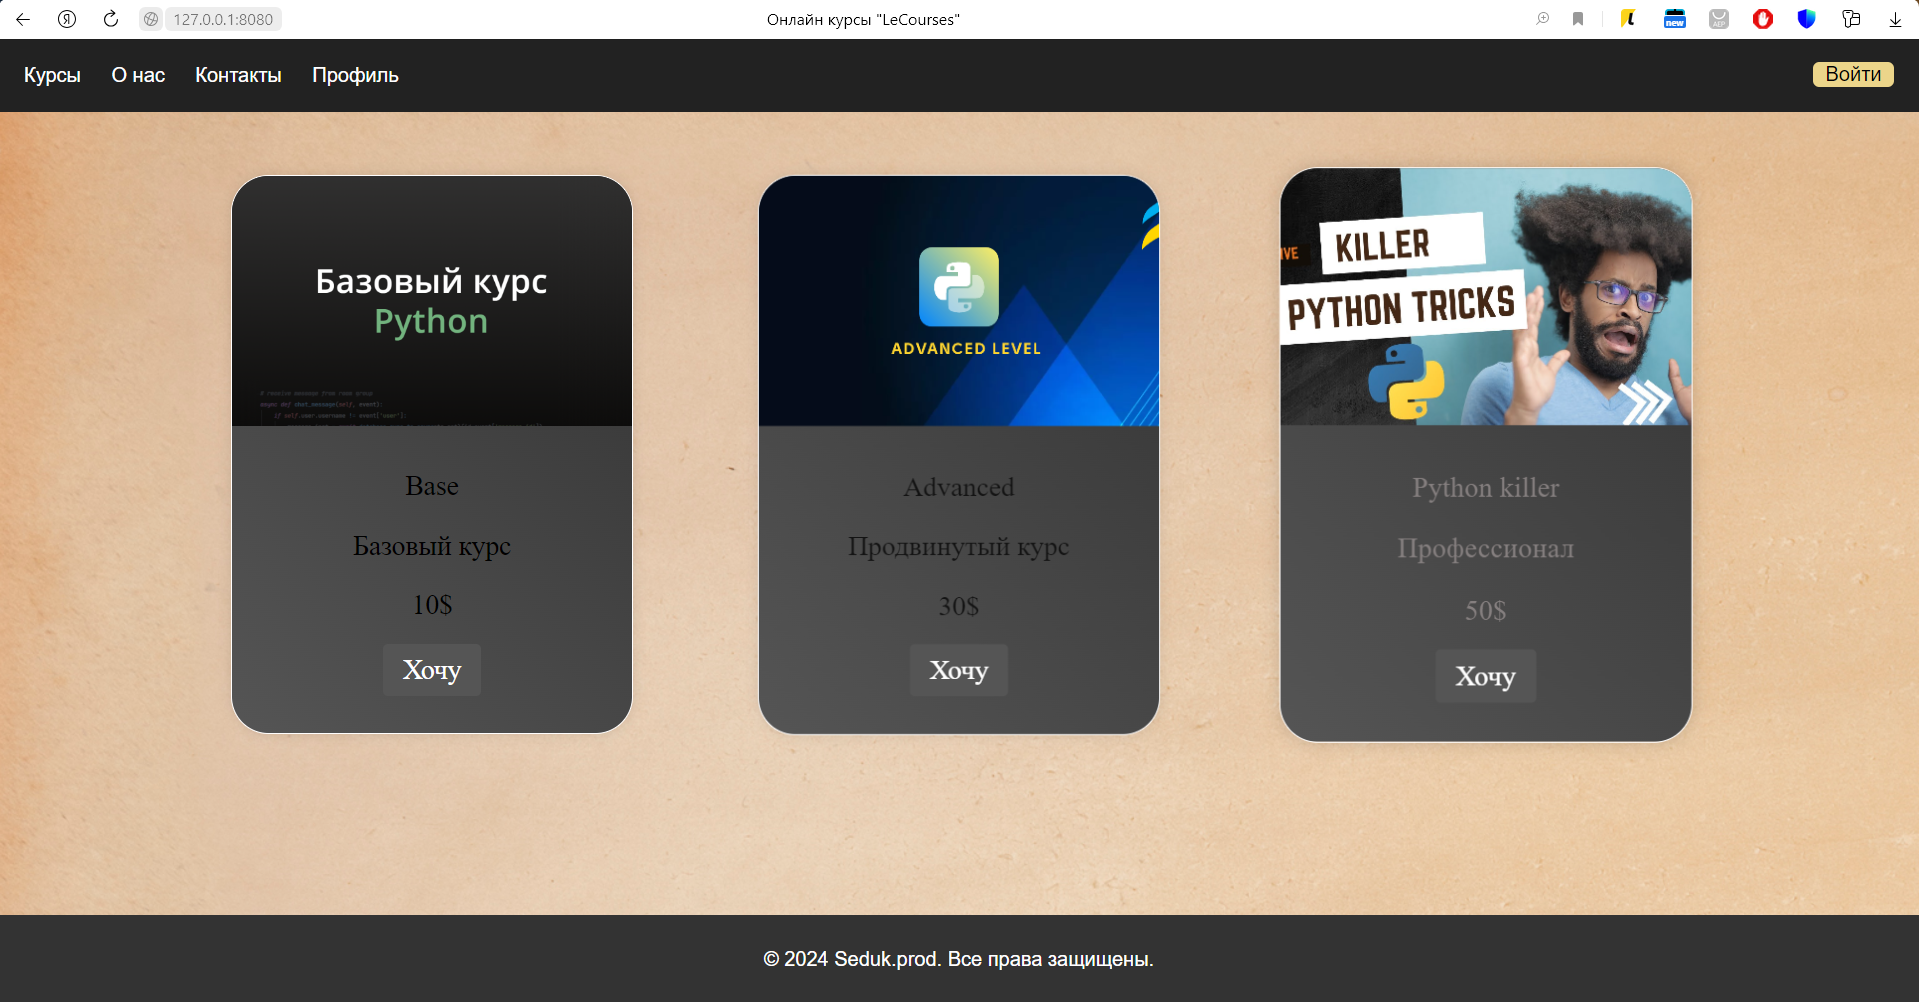
\includegraphics[width=1\linewidth]{main1}}
	\caption{Главная страница сайта курсов}
	\label{main:image}
\end{figure}

На рисунке \ref{menu:image} представлена страница курса.

\begin{figure}[ht]
	\center{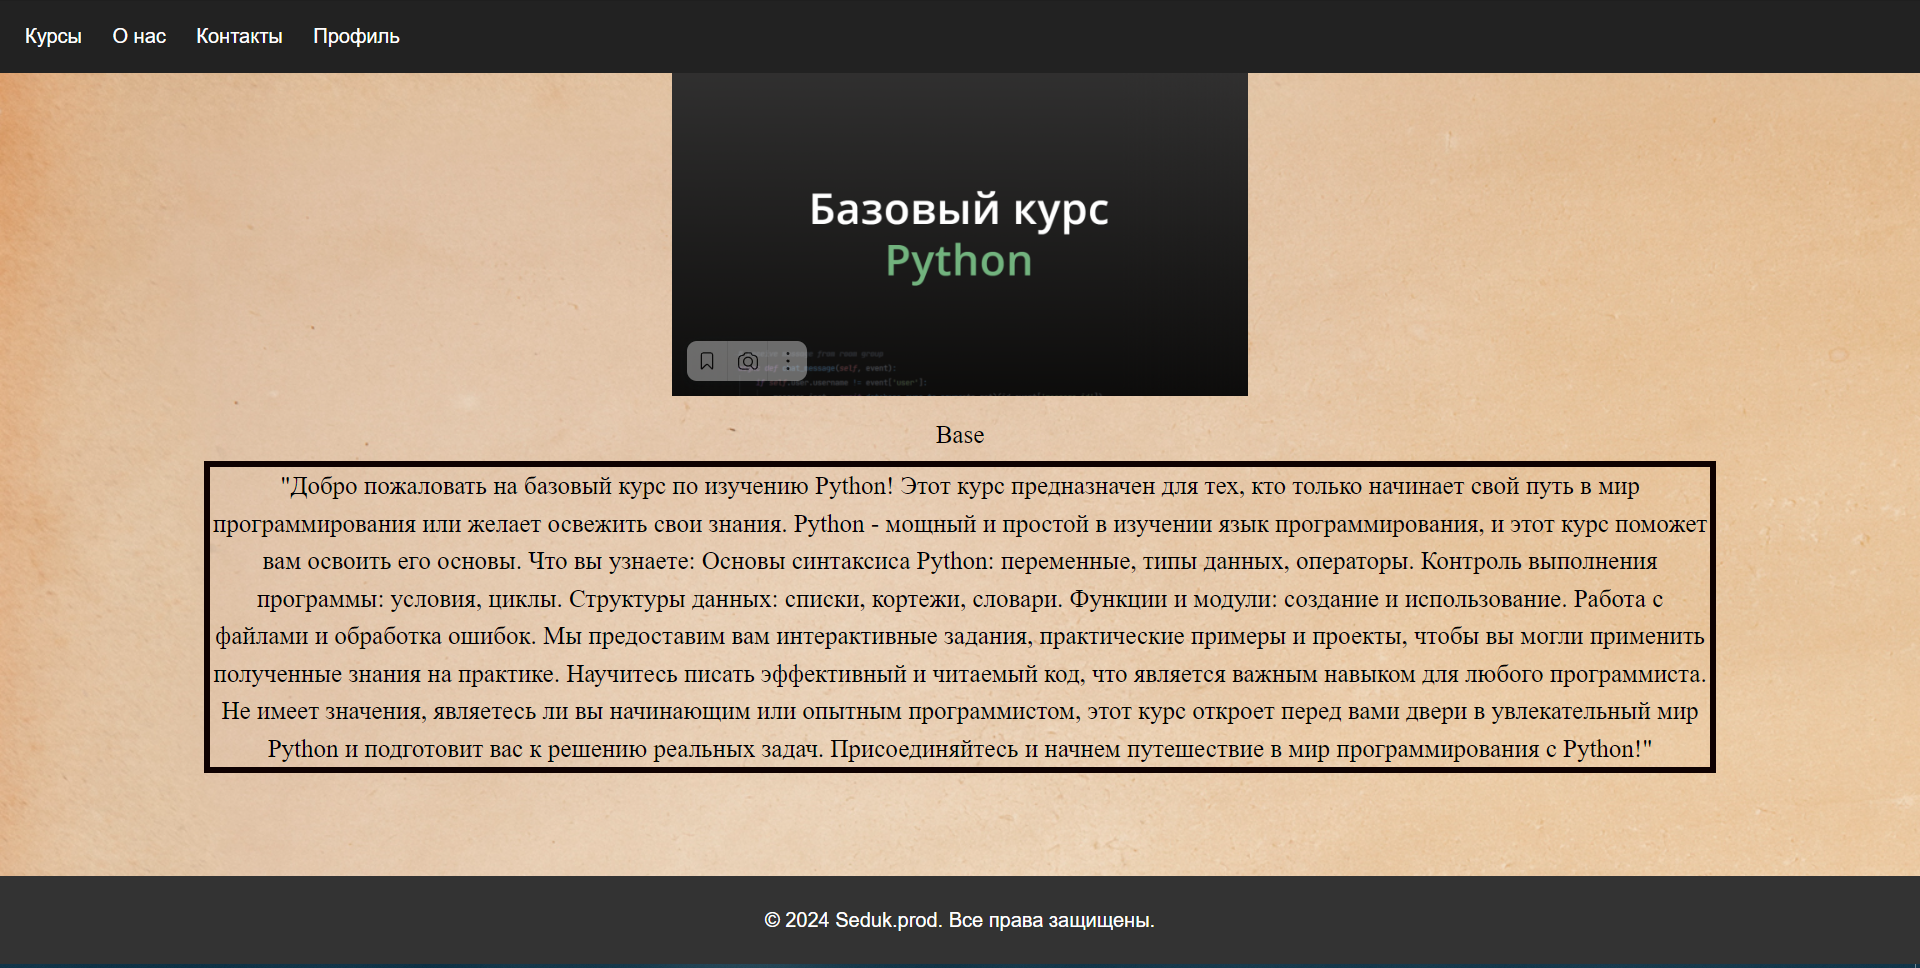
\includegraphics[width=1\linewidth]{menu}}
	\caption{Страница курса}
	\label{menu:image}
\end{figure}

\newpage
На рисунке \ref{enter:image} представлена страница авторизации в профиль.

\begin{figure}[ht]
	\center{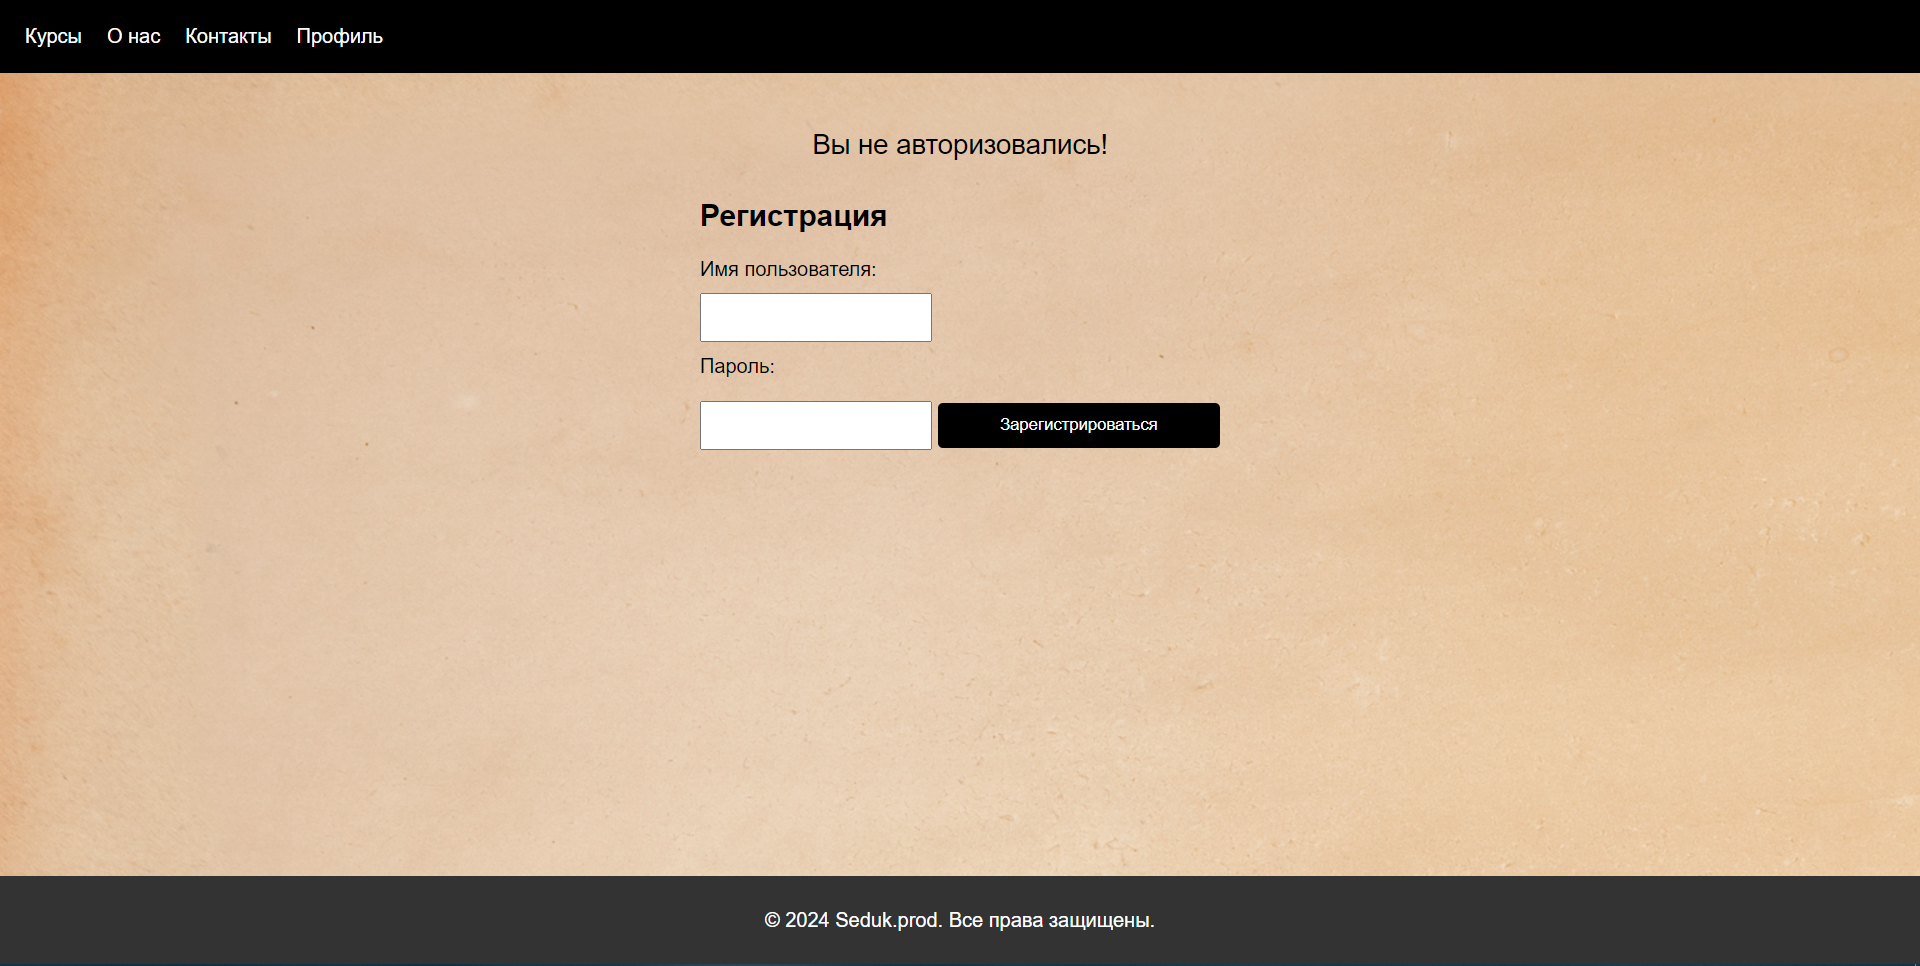
\includegraphics[width=1\linewidth]{enter}}
	\caption{Страница авторизации}
	\label{enter:image}
\end{figure}

На рисунке \ref{pay:image} представлена страница оплаты.

\begin{figure}[ht]
	\center{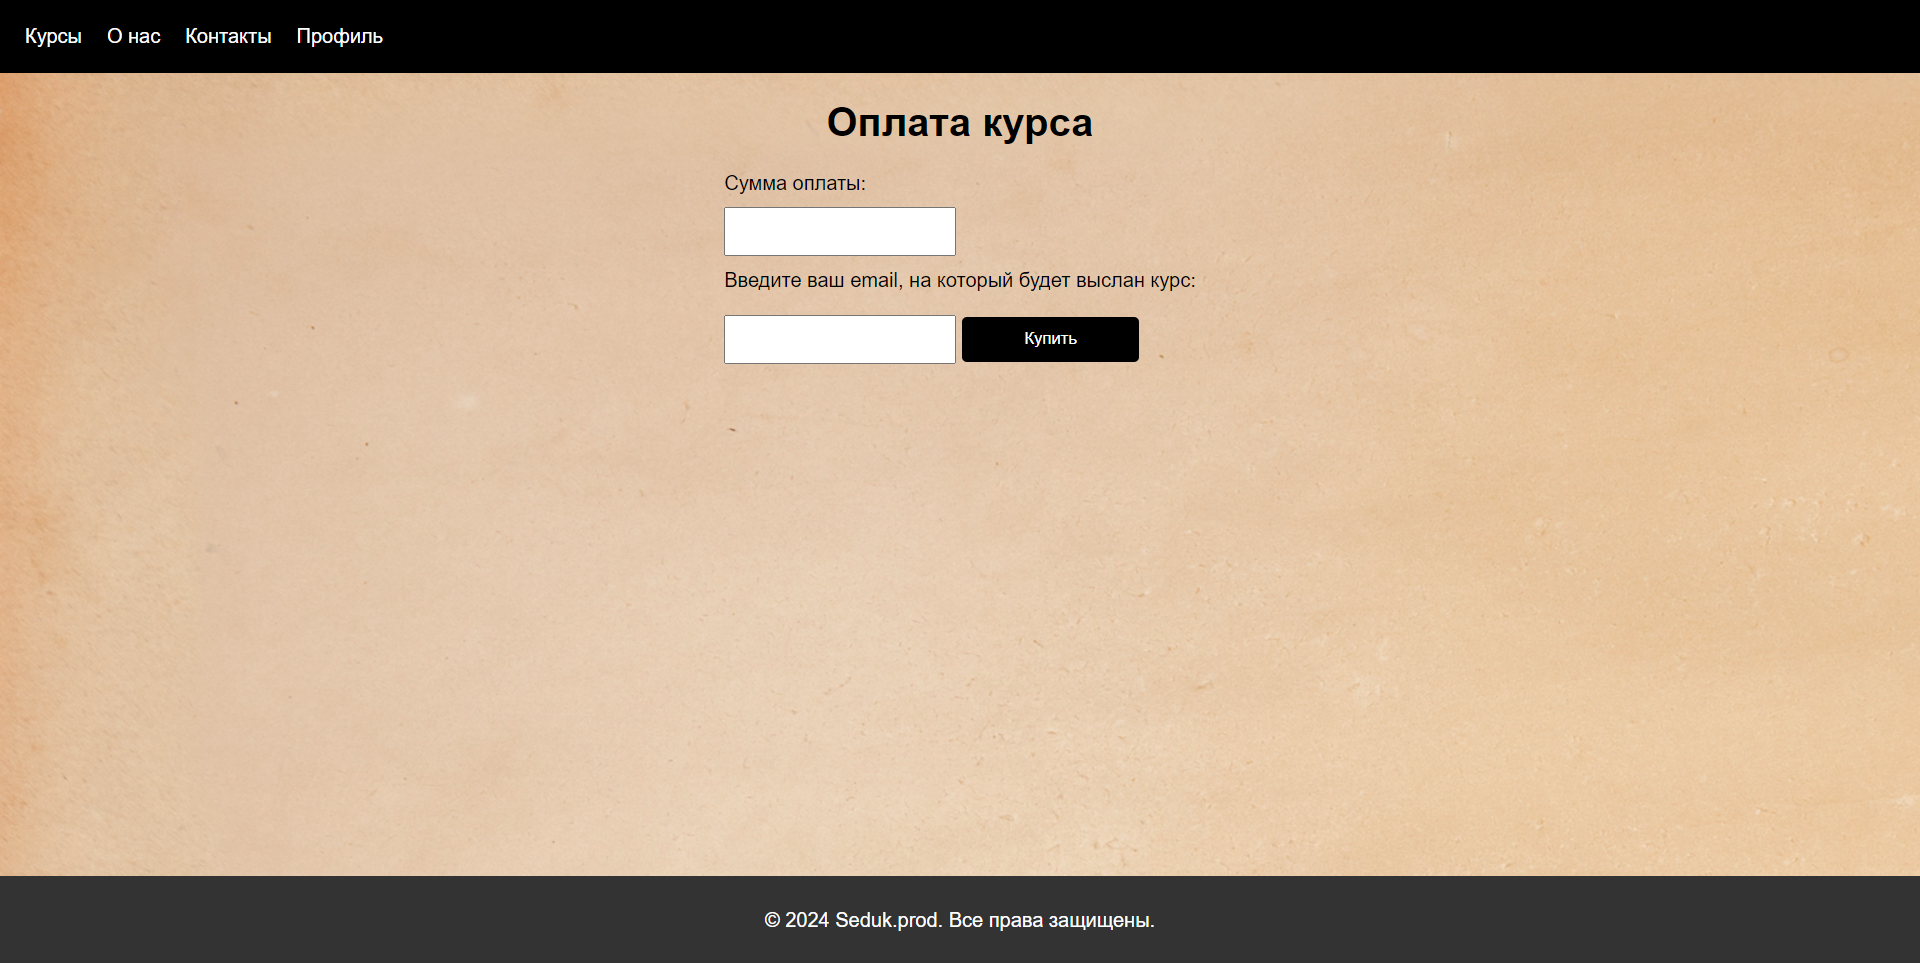
\includegraphics[width=1\linewidth]{pay}}
	\caption{Страница оплаты курса}
	\label{pay:image}
\end{figure}

\newpage
На рисунке \ref{getpay:image} представлена страница успешной оплаты.

\begin{figure}[ht]
	\center{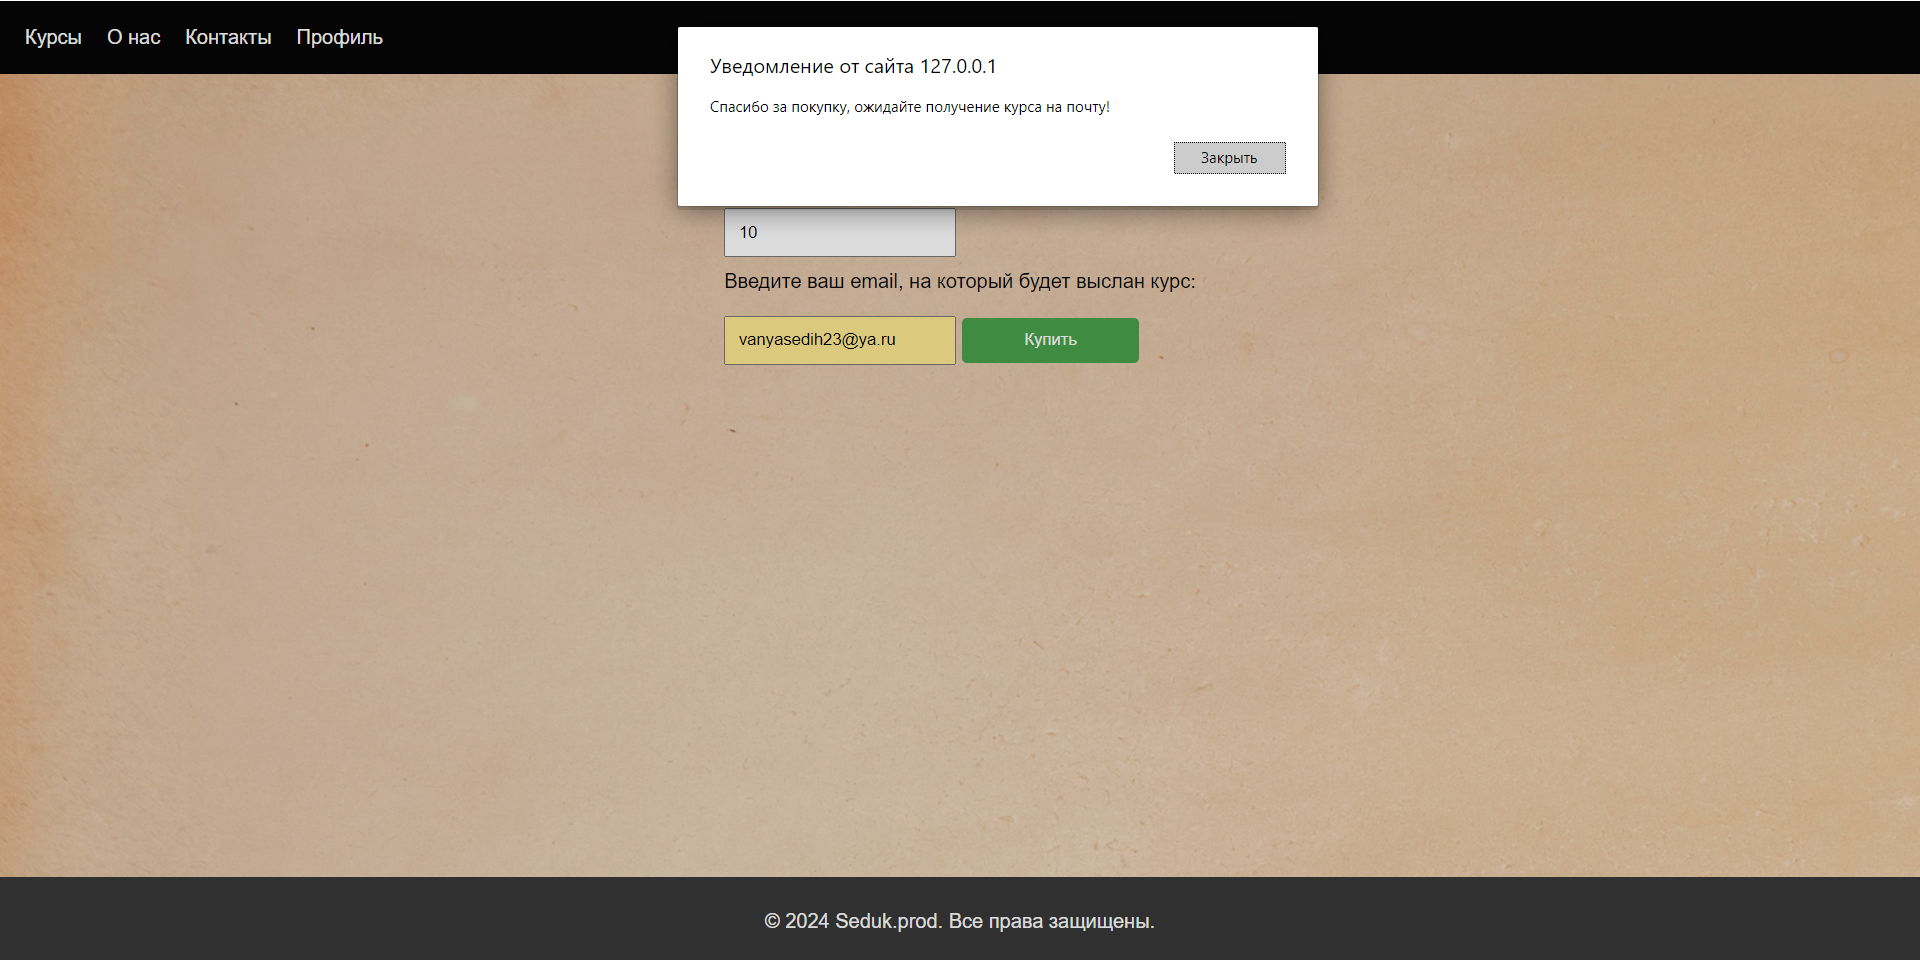
\includegraphics[width=1\linewidth]{getpay}}
	\caption{Страница успешной оплаты}
	\label{getpay:image}
\end{figure}


На рисунке \ref{about:image} представлена страница о нас.

\begin{figure}[ht]
	\center{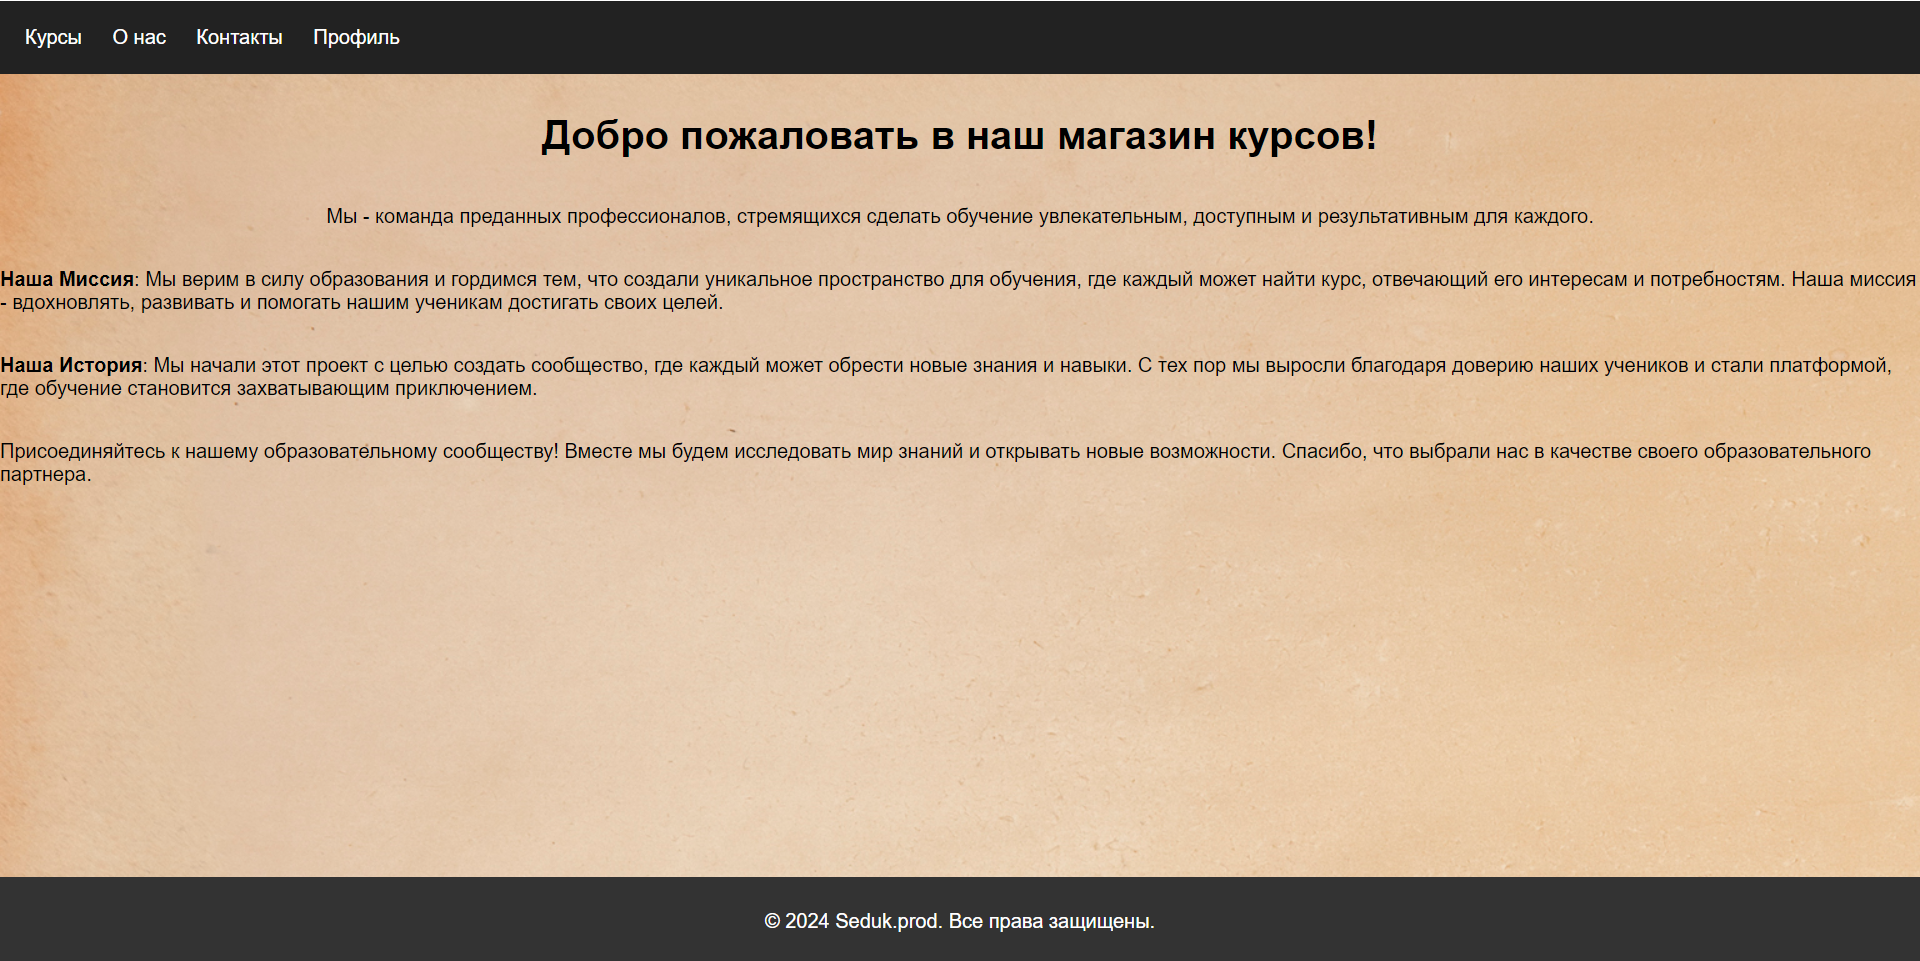
\includegraphics[width=1\linewidth]{about}}
	\caption{Страница о нас}
	\label{about:image}
\end{figure}

\newpage
На рисунке \ref{contact:image} представлена страница контакты.

\begin{figure}[ht]
	\center{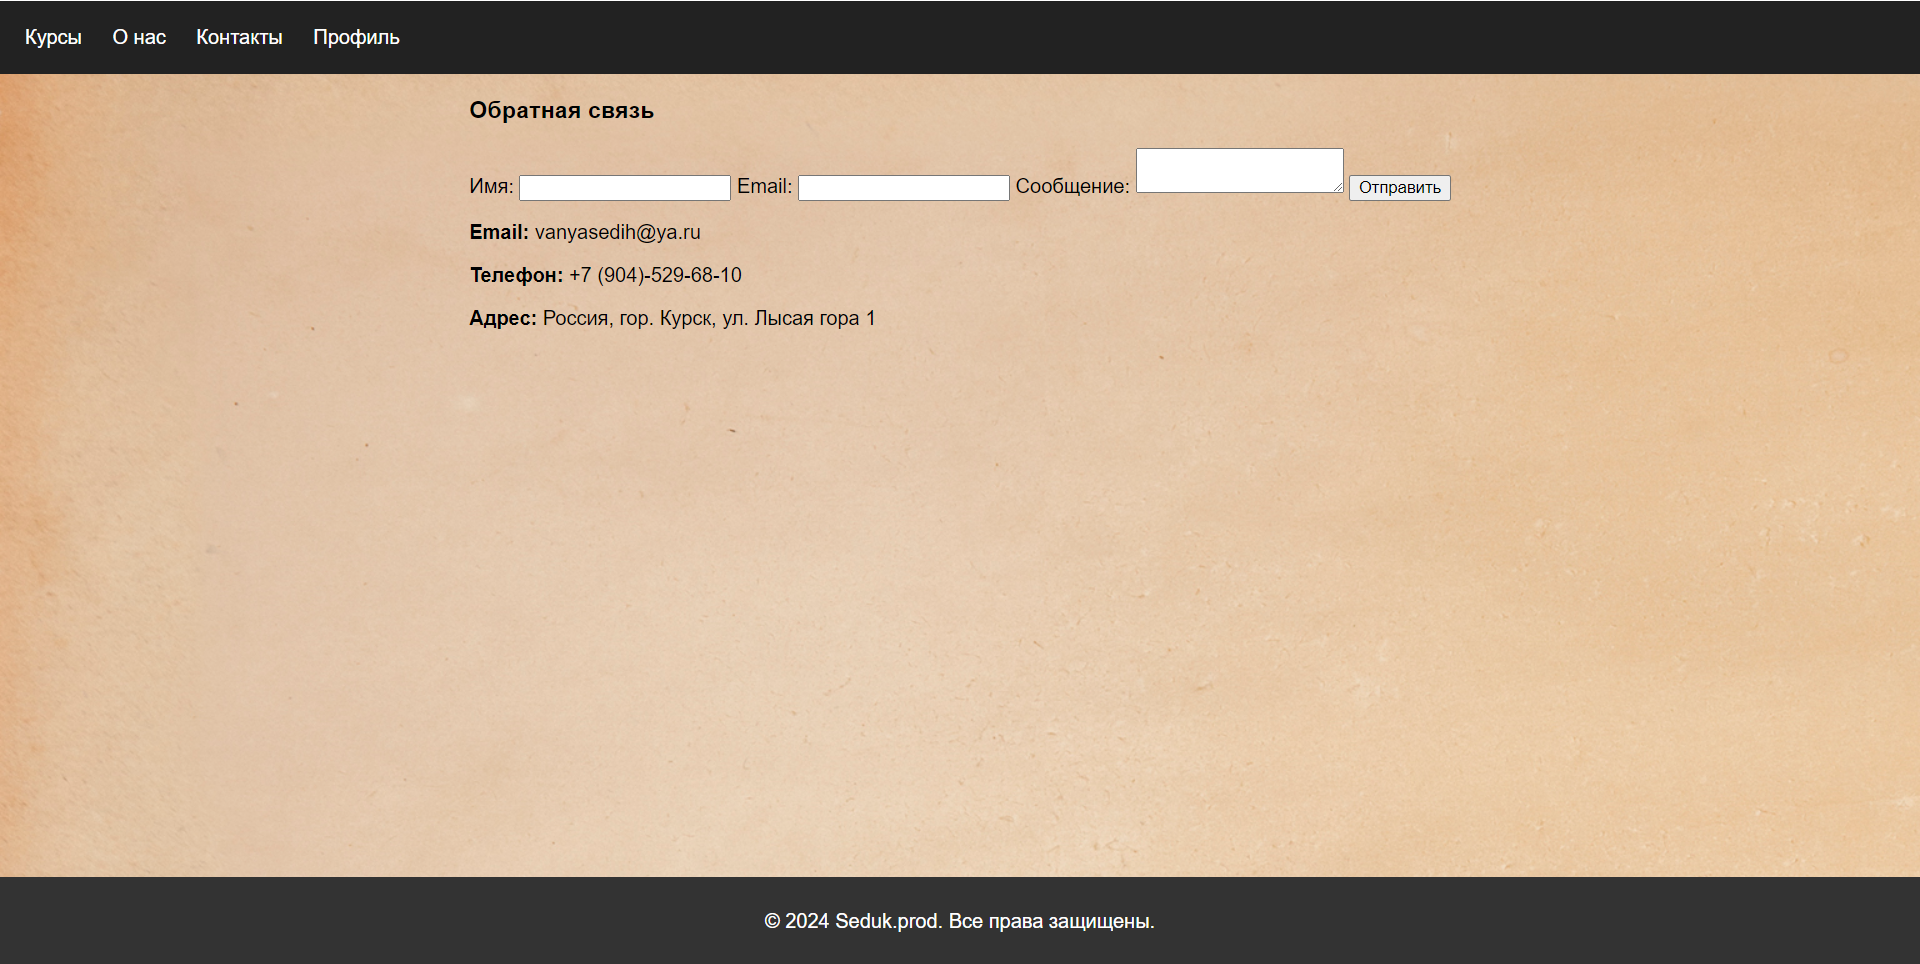
\includegraphics[width=1\linewidth]{contact}}
	\caption{Страница контакты}
	\label{contact:image}
\end{figure}

На рисунке \ref{mess:image} представлена страница отправки обратной связи.

\begin{figure}[ht]
	\center{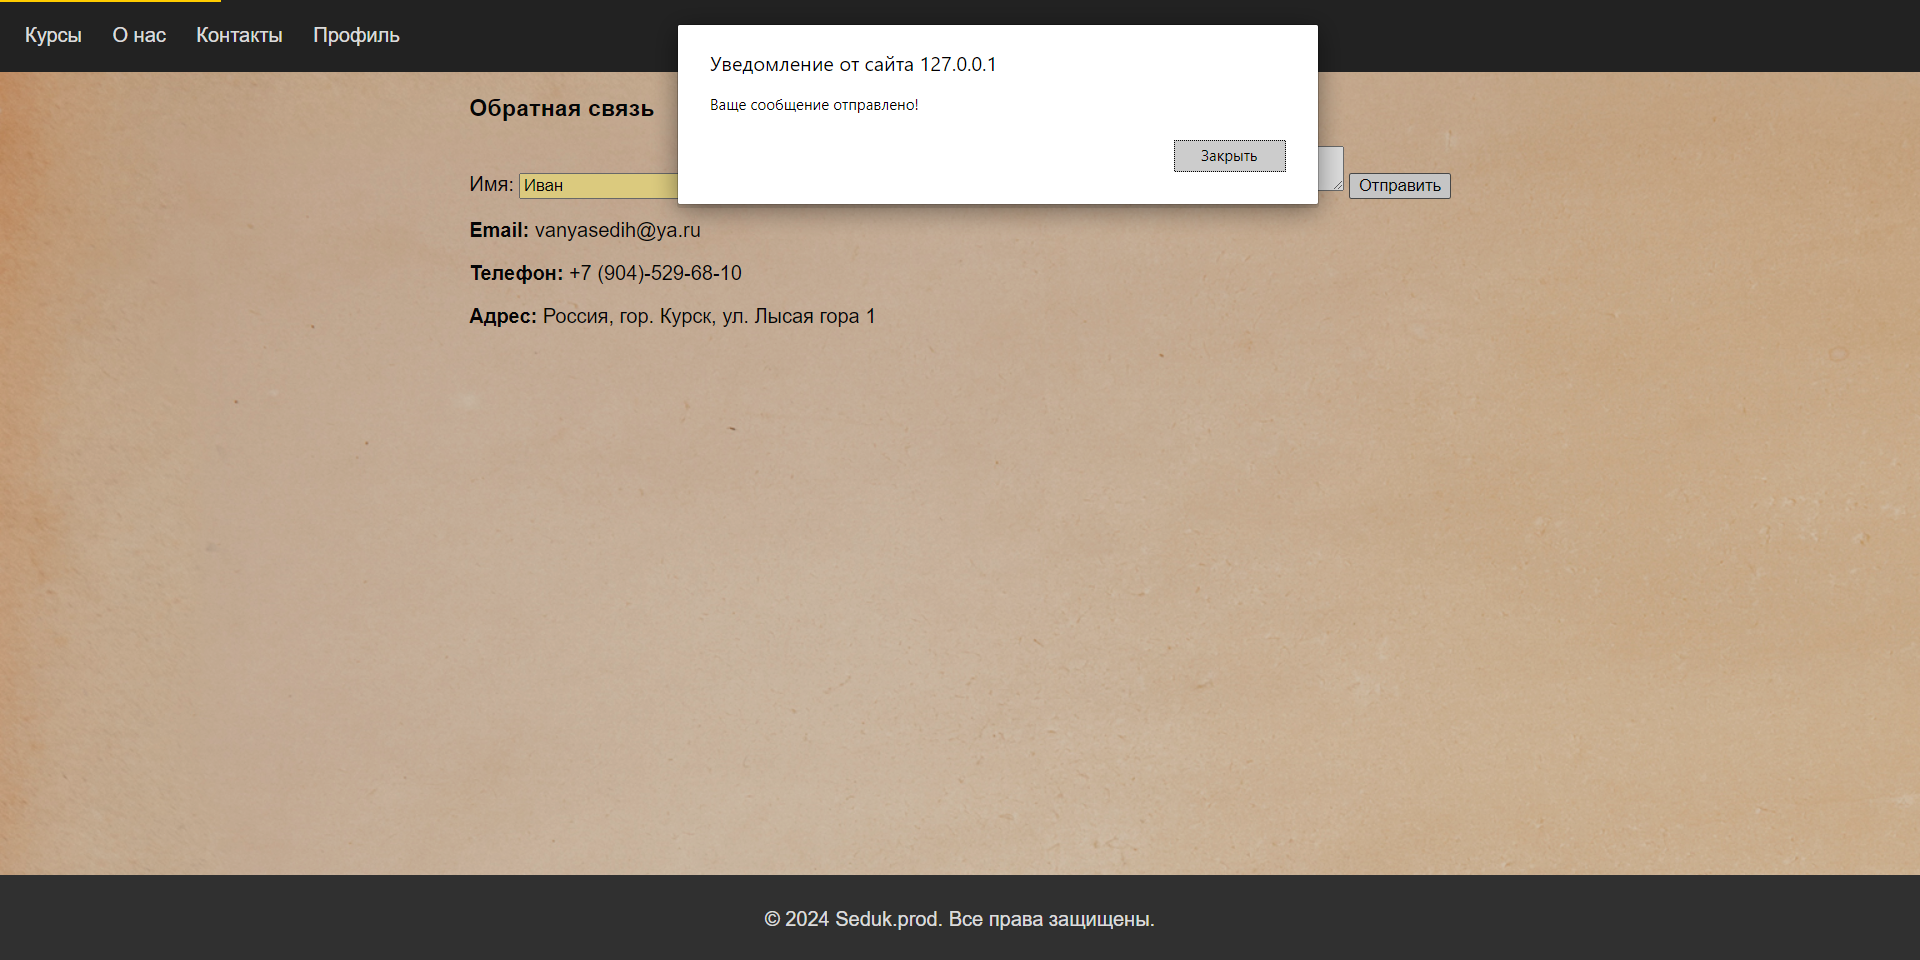
\includegraphics[width=1\linewidth]{mess}}
	\caption{Страница отправки обратной связи}
	\label{mess:image}
\end{figure}

